In this section we provide an overview of PaaS clouds and Cerebro. Then we present a model for 
negotiating response time SLAs for web APIs deployed in PaaS clouds.

PaaS clouds enforce a restricted programming model on the application developer to guarantee
the scalability, security and the availability of the cloud-hosted applications. To begin with,
PaaS clouds provide a predefined set of programming interfaces through which they export 
various platform services. We shall refer to these programming interfaces as the cloud software
development kit (cloud SDK). The cloud SDK exposes scalable functionality that can be used to 
program a wide range of application features. These include key-value data stores, databases, 
caching, task scheduling, and user management. In a typical PaaS environment
such as Google App Engine (or AppScale), the developer must use the cloud SDK to implement
all the required application components and APIs, as the use of third party services or libraries is
restricted within the cloud platform. 

Similarly, PaaS clouds may impose restrictions on performing
certain types of I/O operations, and executing long running tasks. For example, Google App Engine
denies applications access to the local file system (i.e. no file I/O). Furthermore, it forces the
developer to implement all application tasks as request-response interactions of a web service
where all requests must be processed
under 60 seconds. Any task that takes longer than this is terminated by the cloud platform.
This restriction is particularly interesting to us, since it gives a 60 second default SLA
for all web APIs developed for Google App Engine.
The result of all these restrictions is a programming model that is
amenable to reasoning via static analysis; a feature we exploit in the design of Cerebro. By surveying
a collection of open source PaaS applications we have also found that program features that typically
inhibit static analysis (e.g. excessive branching and loops) are scarce among PaaS-hosted
applications.

\begin{figure}
\centering
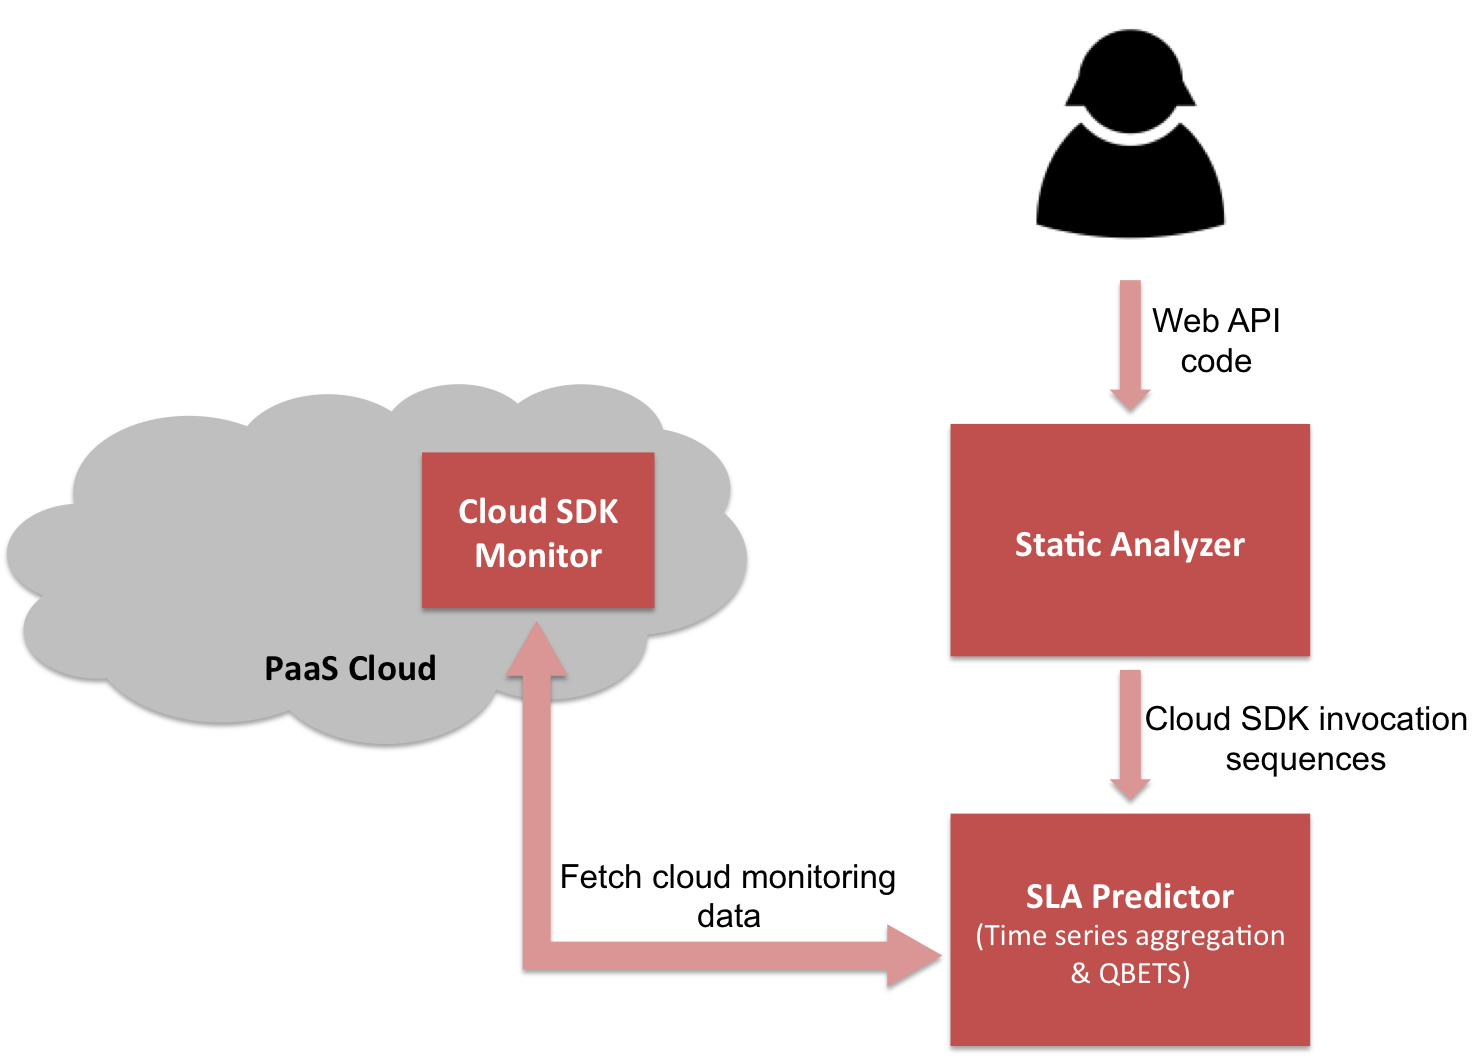
\includegraphics[scale=0.35]{cerebro_arch}
\caption{Main components of Cerebro and their interactions.}
\label{fig:cerebro_arch}
\vspace{-0.2in}
\end{figure}

Figure~\ref{fig:cerebro_arch} illustrates the main components of Cerebro, and how they interact with
each other. It runs a cloud SDK monitor in the PaaS environment, that periodically benchmarks each
SDK operation for its execution time, and records the results as a set of time series (one time series 
per SDK operation). 
This component runs independent of all the applications deployed in the cloud, and it is active as long
as the cloud platform is available for serving requests. 

When an application developer submits a new
application to the cloud platform, Cerebro intercepts it, and runs it through a static analyzer.
Cerebro's static analyzer is designed to extract the sequence of cloud SDK operations invoked by each
of the web API operations in a given application. When the application code contains branches, it
extracts multiple sequences of cloud SDK operations -- one sequence per code path. The static
analyzer also looks for loops, and if SDK operations are embedded within a loop, it attempts to
estimate loop bounds using existing loop bound analysis methods. If it fails, Cerebro prompts the 
application developer to provide a reasonable upper
bound for the loop count. Our survey results show that most of the time when loops are present in
a PaaS application, they simply iterate through a dataset read from the cloud datastore. 
Determining the bounds of such data-dependent loops is equivalent to establishing an upper bound
for the size of the underlying database, which most application developers are capable of performing.